\documentclass{article}
\usepackage[utf8]{inputenc}
\usepackage{tikz}
\usetikzlibrary{mindmap}

\pagestyle{empty}
\begin{document}

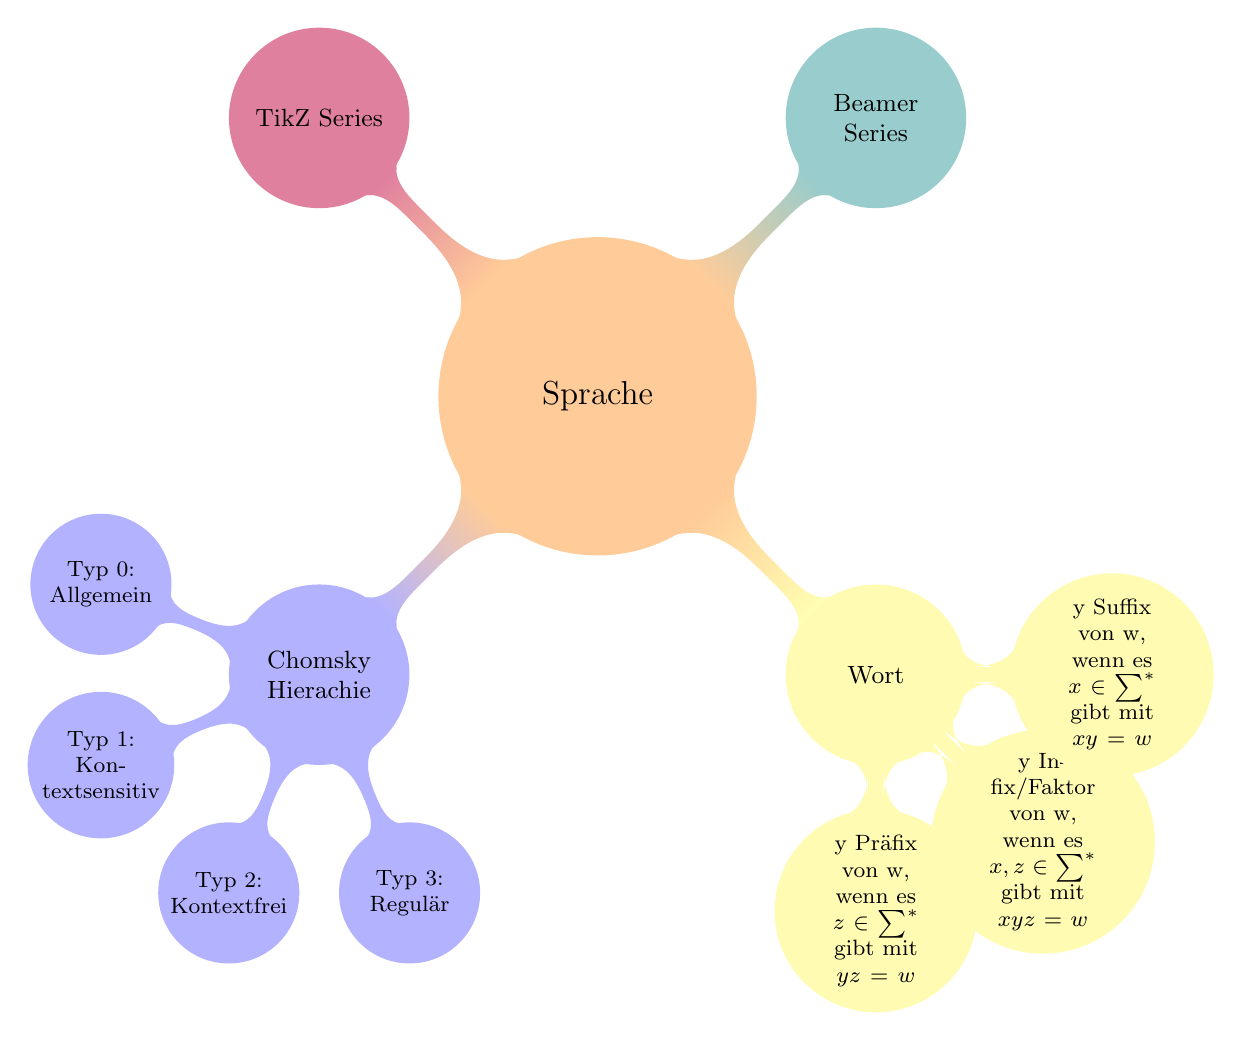
\begin{tikzpicture}[mindmap, grow cyclic, every node/.style=concept, concept color=orange!40,
    level 1/.append style={level distance=5cm,sibling angle=90},
    level 2/.append style={level distance=3cm,sibling angle=45}]

\node{Sprache}
    child [concept color=blue!30] { node {Chomsky Hierachie}
        child { node {Typ 0: Allgemein}}
        child { node {Typ 1: Kontextsensitiv}}
        child { node {Typ 2: Kontextfrei}}
        child { node {Typ 3: Regulär}}
    }
    child [concept color=yellow!30] { node {Wort}
        child { node { y Präfix von w, wenn es $z\in\sum^*$ gibt mit $yz=w$}}
        child { node { y Infix/Faktor von w, wenn es $x,z\in\sum^*$ gibt mit $xyz = w$}}
        child { node { y Suffix von w, wenn es $x\in\sum^*$ gibt mit $xy=w$}}
    }
    child [concept color=teal!40] { node {Beamer Series}
    }
    child [concept color=purple!50] { node {TikZ Series}
    };
\end{tikzpicture}

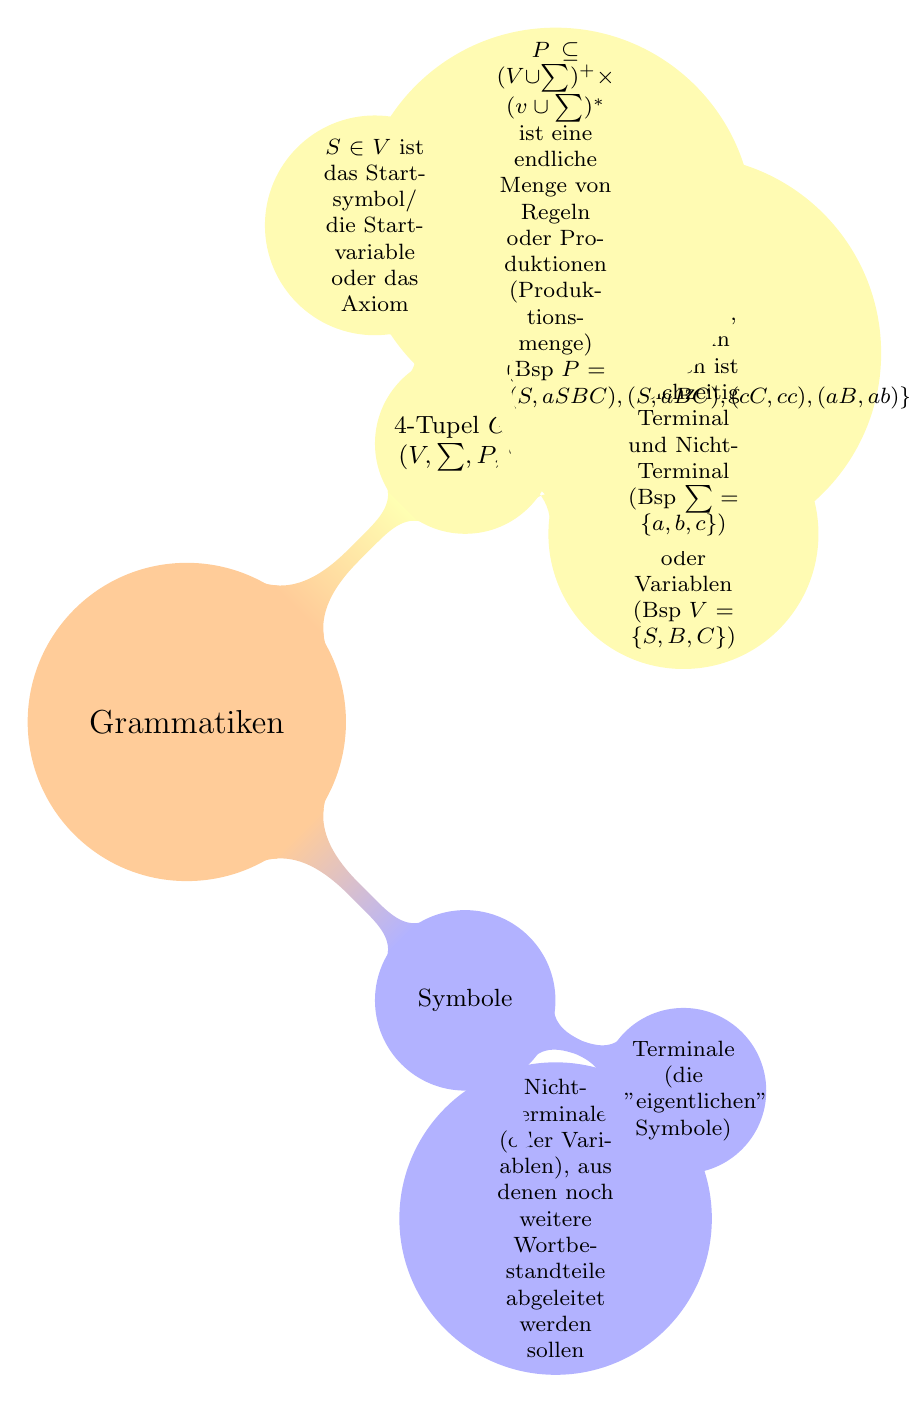
\begin{tikzpicture}[mindmap, grow cyclic, every node/.style=concept, concept color=orange!40,
    level 1/.append style={level distance=5cm,sibling angle=90},
    level 2/.append style={level distance=3cm,sibling angle=45}]
\node{Grammatiken}
    child [concept color=blue!30] { node {Symbole}
        child { node {Nicht-Terminale (oder Variablen), aus denen noch weitere Wortbestandteile abgeleitet werden sollen}}
        child { node {Terminale (die "eigentlichen" Symbole)}}
    }
    child [concept color=yellow!30] { node {4-Tupel $G=(V,\sum, P, S)$}
        child { node {V ist eine endliche Menge von Nicht-Terminalen oder Variablen (Bsp $V=\{S,B,C\}$)}}
        child { node {$\sum$ ist ein Alphabet (Menge der Terminale) mit $V\cap \sum= \varnothing$, d.h. kein Zeichen ist gleichzeitig Terminal und Nicht-Terminal (Bsp $\sum=\{a,b,c\}$)}}
        child { node {$P\subseteq (V\cup \sum)^+ \times (v\cup\sum)^*$ ist eine endliche Menge von Regeln oder Produktionen (Produktionsmenge) (Bsp $P=\{(S,aSBC), (S,aBC), (cC,cc), (aB,ab)\}$)}}
        child { node {$S\in V$ ist das Startsymbol/ die Startvariable oder das Axiom}}
    }
    ;
\end{tikzpicture}

\end{document}
